% NOTE: This section needs most references, theoretical citations, etc.
\section{Architecture}
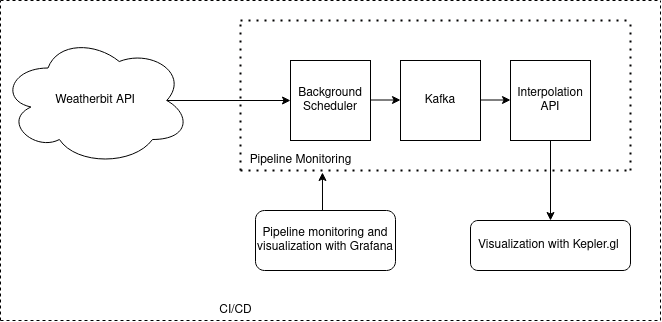
\includegraphics[width=\linewidth]{figures/architecture.png}
\subsection{Overview}
When designing the system architecture for this project, our objective was to utilize many of the technologies and frameworks we have discussed throughout the semester.
With that in mind, we decided to approach each portion of our system as a micro-service that could be easily containerized and managed by a container orchestration service.
In doing so, we have designed a system that attempts to be both resilient and highly available. 

\subsection{Producer}
Much of this project relies on geospatial data.
Namely, we utilized live weather data served from a data vendor Weatherbit.io \cite{weatherbit}.
Our producer uses a background scheduler that periodically polls weatherbit's API to retrieve the current weather.
These polls occur every 15 minutes (the minimum possible interval new data is guaranteed).
To make this data available to the rest of our services, we utilized Kafka.
We published this data to the Kafka brokers, encoding the topics to reflect the location of the weather station from which they were received.

\subsection{Broker}
Since we are using live data, we wanted to quickly send our data to the end application with very little latency. 
In the 'Principles of Cloud Computing' course, we often dumped data to a database and then continued processing the data in another service by querying the database.
The issue with this approach is that one incurs a significant cost of reads and writes to said database \cite{stonebraker20058}.
However, we still wanted to process a subset of generated data, not necessarily all at once, requiring a query-like operation.
We chose to use a publish and subscribe broker,
with an encoded topic for each weather station so that our front-end application could only subscribe to the necessary station feeds. 
The GPS coordinates of the station encoded the weather station topics.
A better choice for our architecture would have been to use a streaming service instead of a publish and subscribe broker. 
The primary reason is one could more easily query the data stream, giving the benefits of both a database and stream processing.
However, due to time constraints to learn a new framework and the fact we could accomplish a pseudo-query, we found the publish-subscribe model sufficient. 

\subsection{RESTful API}
The RESTFul API connects the front-end dashboard with the data pipeline. 
The notable aspects of the API are that it processes the data and then sends back the interpolated data to the front-end dashboard. 

\subsection{Web Application}
Including a web application provides meaningful visualizations of interpolated data to showcase the technical aspects of the project. 
Containerization is an essential requirement for the web application so that it is deployed as a remote web service,
but could also be run locally if the cost of a performant instance was too high. 
Since locally running a web application can be problematic if all dependencies are not installed,
or a user uses a non-Linux system,
containerization ensures operatability. 

\subsection{CI/CD}
One of our goals for this project was high availability. To achieve this, we needed to implement a CI/CD pipeline. We utilized Jenkins, an open-source DevOps tool designed explicitly for managing CI/CD pipelines. If any new changes are observed on any branch, the code is built and tested to ensure that the new version is successful before sending it to production. Jenkins runs inside a Docker container and is hosted on an AWS EC2 instance. It scans the repository every 2 minutes and looks for new commits. If a new commit is detected, the commit is built, and tests are run to ensure that the new version works as expected.

\subsection{Container Orchestration}
The primary reason for using container orchestration is we wanted a controller that monitors the current state versus the desired state, taking action to converge these states if a failure causes divergence \cite{burns2016borg}.
A controller pattern can be complicated and time-intensive to implement,
but when services are containerized and programmed through declarative language, 
we can gain a lot of resiliency at little cost.